% Chapter 14

\chapter{Determination of quark fragmentation functions into kaons} % Chapter title

\label{ch:FF} % For referencing the chapter elsewhere, use \autoref{ch:name}

%----------------------------------------------------------------------------------------

In the previous chapter, we obtained charged kaon multiplicities $M^K(x,Q^2,z)$. As these multiplicities can be expressed as a combination of the PDFs $q(x,Q^2)$ and the FFs $D^K_q(z,Q^2)$, assuming that the PDFs are known, they can be used to extract the quark fragmentation functions into kaon.


%----------------------------------------------------------------------------------------

\section{LO QCD fit of kaon multiplicities}

$D^K$ can be obtained from a pQCD fit to the existing multiplicities. While DSEHS or JAM are doing such studies in NLO, in COMPASS only a LO QCD code is available. The extraction of FFs from the measured $K^{\pm}$ multiplicities is performed in a LO pQCD fashion according to Eq.~\ref{eq:MultpQCD}:
%
\begin{equation}
  \frac{dM^h(x,Q^2,z)}{dz} = \frac{d^3\sigma^h(x,Q^2,z)/dxdQ^2dz}{d^3\sigma^{DIS}(x,Q^2,z)/dxdQ^2} = \frac{\sum_q e^2_q(x,Q^2)D^h_q(z,Q^2)}{\sum_q e^2_qq(x,Q^2)},
\end{equation}
%
with $q(x,Q^2)$ are the quark PDFs for the flavour $q$. Using a standard $\chi^2$ minimization over the data points with the minimization framework Minuit2 of the ROOT package:
%
\begin{equation} \label{eq:MultpQCD}
  \chi^2 = \sum_j \frac{\left[T_j\left(x_j,Q^2_j,z_j\right) - M_j\left(x_j,Q^2_j,z_j\right)\right]^2}{\sigma^2_j},
\end{equation}
%
where $M_j$ are the measured multiplicities and $\sigma^2_j$ are the quadratic sum of the statistical errors. $T_j$ are the multiplicities evaluated for a set of parameters for a given parametrisation. Due to the large $Q^2$ span covered by the data, it is mandatory to properly take into account the $Q^2$ dependence of FFs and PDFs. Thus the $T_j$ are evaluated at $Q^2_0$ = 1 (GeV/$c$)$^2$ and evolved to their actual $Q^2_j$ using the LO DGLAP $Q^2$ evolution code provided by M. Hirai and S. Kumano \cite{HKNS}.

As described in Chapter~\ref{ch:thfw}, four independent FFs (see Eq.~\ref{eq:FFKaon}) are extracted: $D^K_{fav}$, $D^K_{unf}$, $D^K_{s}$ and $D^K_{g}$.
For the current analysis, the following parametrization, similar to the one from DSEHS described in Chapter~\ref{ch:thfw} is used:
%
\begin{equation}
  \begin{split}
    zD_i(z,Q^2_0) = \frac{N_i z^{\alpha_i} (1-z)^{\beta_i} (1+\gamma_i(1-z)^{\delta_i})}{\int_{0.2}^{0.85} z'^{\alpha_i} (1-z')^{\beta_i} (1+\gamma_i(1-z')^{\delta_i} dz'},\,i=\{fav\} \\
    zD_i(z,Q^2_0) = \frac{N_i z^{\alpha_i} (1-z)^{\beta_i}}{\int_{0.2}^{0.85} z'^{\alpha_i} (1-z')^{\beta_i} dz'},\,i=\{s,unf,g\}.
  \end{split}
\end{equation}
%
The PDFs set from MSTW$08$ in LO pQCD \cite{MSTW08}, stored by the LHAPDF data group \cite{LHAPDF} was chosen.

\section{Uncertainties calculation}

The statistical and systematic uncertainties of the extracted FFs are determined by using a bootstrap method \cite{replicas}. Therefore a number of resamples of the original multiplicity data are constructed. For each resample the data points are fluctuated proportional to their uncertainty, resulting in a set of data points:
%
\begin{equation}\label{eq:replica}
  M'_j = M_j + R \cdot \sigma_j,
\end{equation}
%
where $M_j$ and $\sigma_j$ are the original value and the corresponding uncertainty of data point $j$, respectively. The factor $R$ is a Gaussian randomly distributed value in the range [$-\infty,\infty$]. Its determination is differently treated for statistical and systematic uncertainties.
The statistical uncertainties are uncorrelated and the deviation of each data point $j$ is calculated with an individual random value $R_j$. Thus, for statistical uncertainties, Eq.~\ref{eq:replica} can be written as:
%
\begin{equation}\label{eq:replica}
  M'_{j,stat} = M_j + R_j \cdot \sigma_{j,stat}.
\end{equation}
%
For systematic uncertainties, for each resample only one random value $R'$ of the standard Gaussian distribution is generated:
%
\begin{equation}\label{eq:replica}
  M'_{j,sys} = M_j + R' \cdot \sigma_{j,sys}.
\end{equation}
%
For both statistical and systematic uncertainties, a set of $100$ resamples is created. Then for each resample the fit is performed as it is done for the original data. To calculate the uncertainty bands, for each $z$ bin, the mean and the RMS values are calculated from the resulting FFs. The uncertainties are centered around the mean value and have the width of the corresponding RMS value.

\section{Kaon fragmentation functions}

The final parameters of the fit are displayed in Table~\ref{tab:Fitparam}. The $\chi^2$ per degrees of freedom for the results is 3.5. A similar fit has been performed with COMPASS data on isoscalar target (see Appendix~\ref{app:Fit}). In Fig.~\ref{pic:FFFit}, the four FFs are shown. The values obtained are significantly higher for $\D{K}{fav}$ and $\D{K}{unf}$ compared to DSS'07 LO results and in agreement with the LO fit of COMPASS data on isoscalar target, while for $\D{K}{str}$ the values are much smaller than DSS'07 LO for both sets. This needs a more detailed investigation and also a fit in NLO. The reason I chose the DSS$07$ fit and not a newer one is that this is the only fit of DSS/DSEHS that is done at LO and it makes more sense to compare LO order extraction than for example LO versus NLO. The fragmentation functions are calculted up to $z = 0.85$ and in the previous chapter, we saw that pQCD is not describing the ratio of charged kaons for $z$ above $0.7$. In this thesis it was assumed that this region is not contraining much the fit hence it should not be a problem but future work should perform a close examination.

These results point out that there is a bad sensitivity of these proton target measurements to the strange quark. In fact these measurement are $u$ dominated and go down to $x\sim10^{-2}$ only, thus is not probing far into the sea. There is not enough sensitivity to the three fragmentation functions to kaons favoured, unfavoured and strange (the gluon FF is not considered as in LO it only comes from the DGLAP evolution). A more refined analysis of COMPASS plus HERMES data taking into account our findings on the multiplicity ratio is needed. An extension of this study would be to do a $K^0$ analysis, which would bring a sample with an extended kinematic range and with independent equation, to study whether it improves the fit. For COMPASS data on isoscalar target such study was conducted but was not conclusive as the $K^0$ sample was not good enough due to reinteractions in the isoscalar target. In the pure proton target there are no such reinteractions, hence the $K^0$ sample needs smaller corrections.

\begin{table}[!h]
  \begin{center}
    \begin{tabular}{ | c | c c c c c | }
      \hline
      \hline
       & N & $\alpha$ & $\beta$ & $\gamma$ & $\delta$ \\
      \hline
      \hline
      $\D{K}{fav}$ & 0.0647 $\pm$ 0.0007 & -1.2 $\pm$ 0.2 & 0.46 $\pm$ 0.07 & -1.6 $\pm$ 0.7 & 3.4 $\pm$ 0.2 \\
      $\D{K}{s}$ & 0.03 $\pm$ 0.01 & 14 $\pm$ 7 & 27 $\pm$ 10 & - & -  \\
      $\D{K}{unf}$ & 0.005 $\pm$ 2 & 4 $\pm$ 5 & 19 $\pm$ 10 & - & - \\
      $\D{K}{glu}$ & 0.08 $\pm$ 0.1 & 16 (fixed) & 11 (fixed) & - & - \\
      \hline
      \hline
    \end{tabular}
  \end{center}
  \caption{Fit parameters for $Q^2_0$ = 1 (GeV/$c$)$^2$. The associated $\chi^2$ is of 3.5.}
  \label{tab:Fitparam}
\end{table}


\begin{figure}[!h]
  \centering
	\subfloat[$zD^{K}_{fav}$]{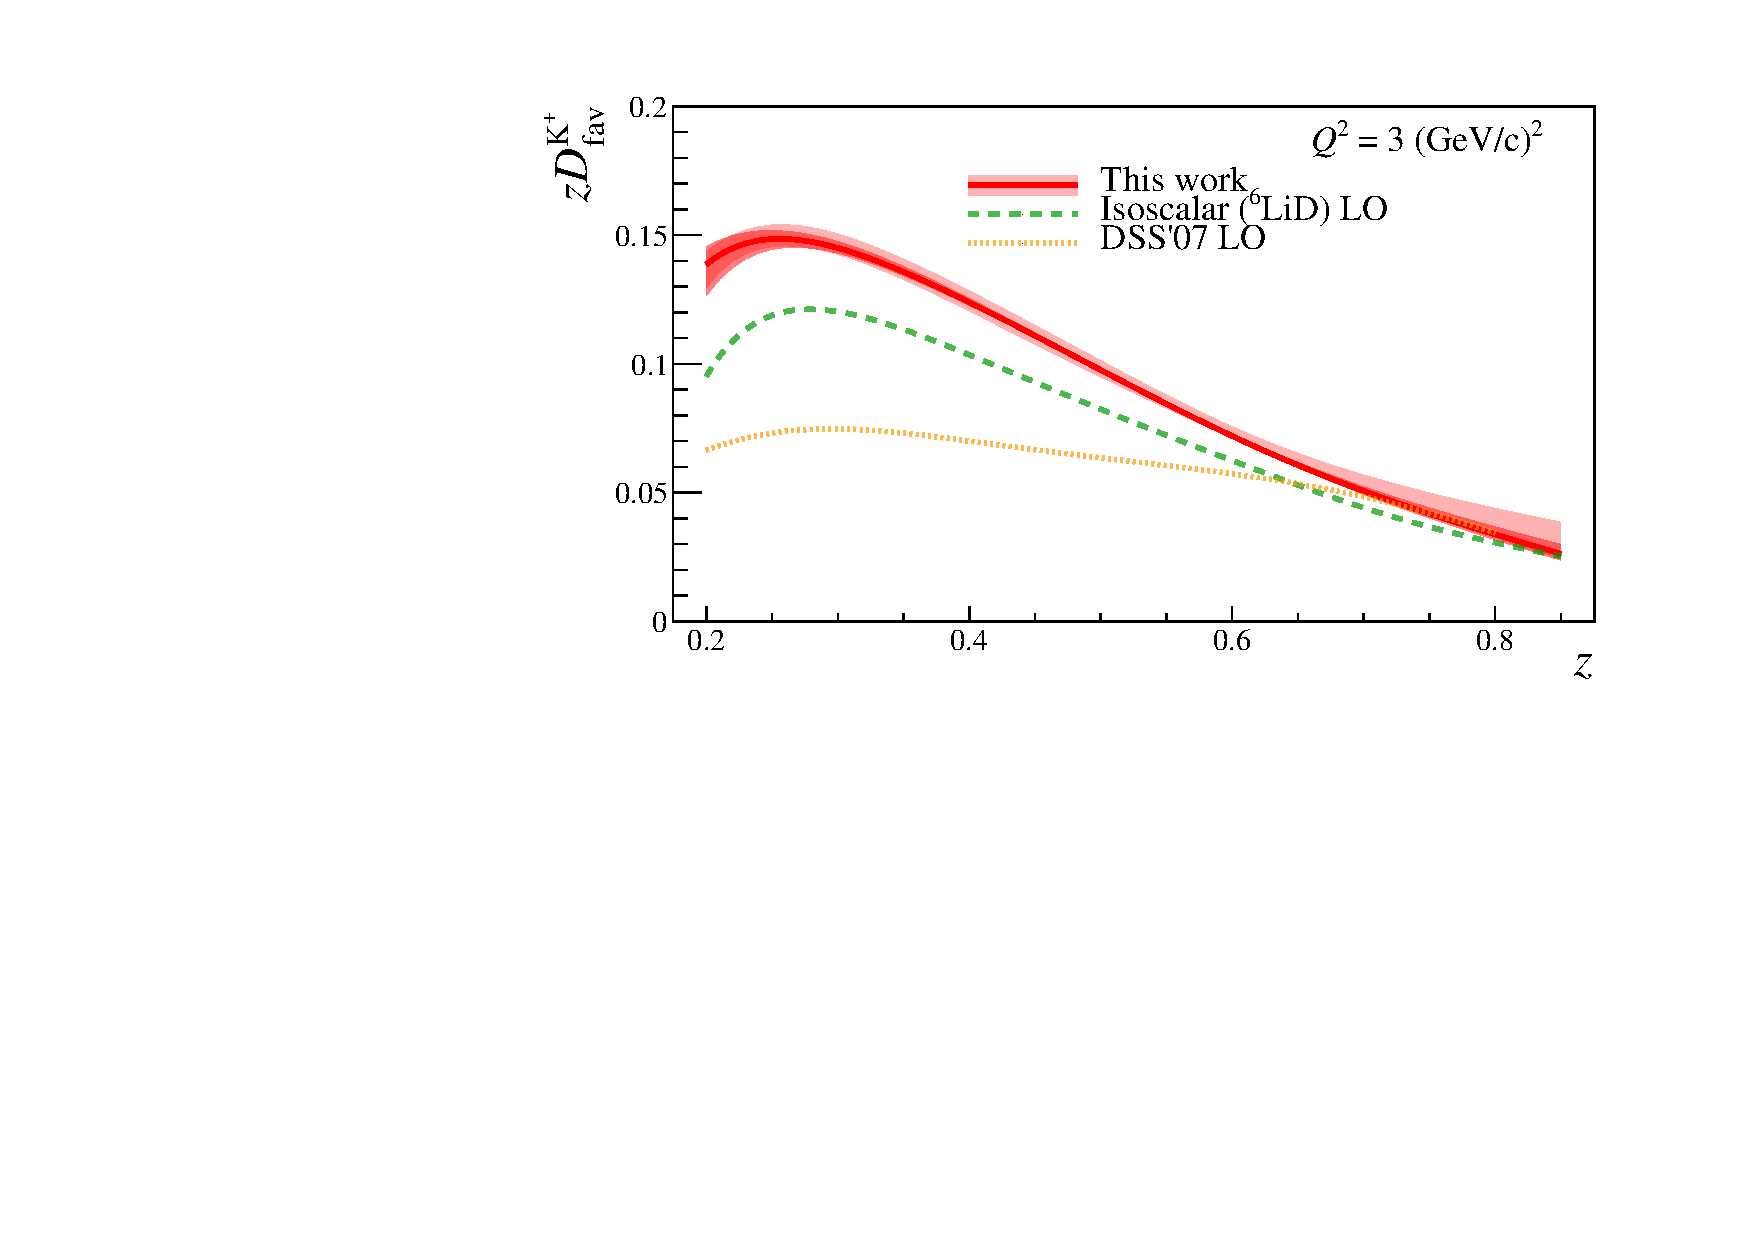
\includegraphics[scale=0.4]{./gfx/fav.pdf}}
  \subfloat[$zD^{K}_{unf}$]{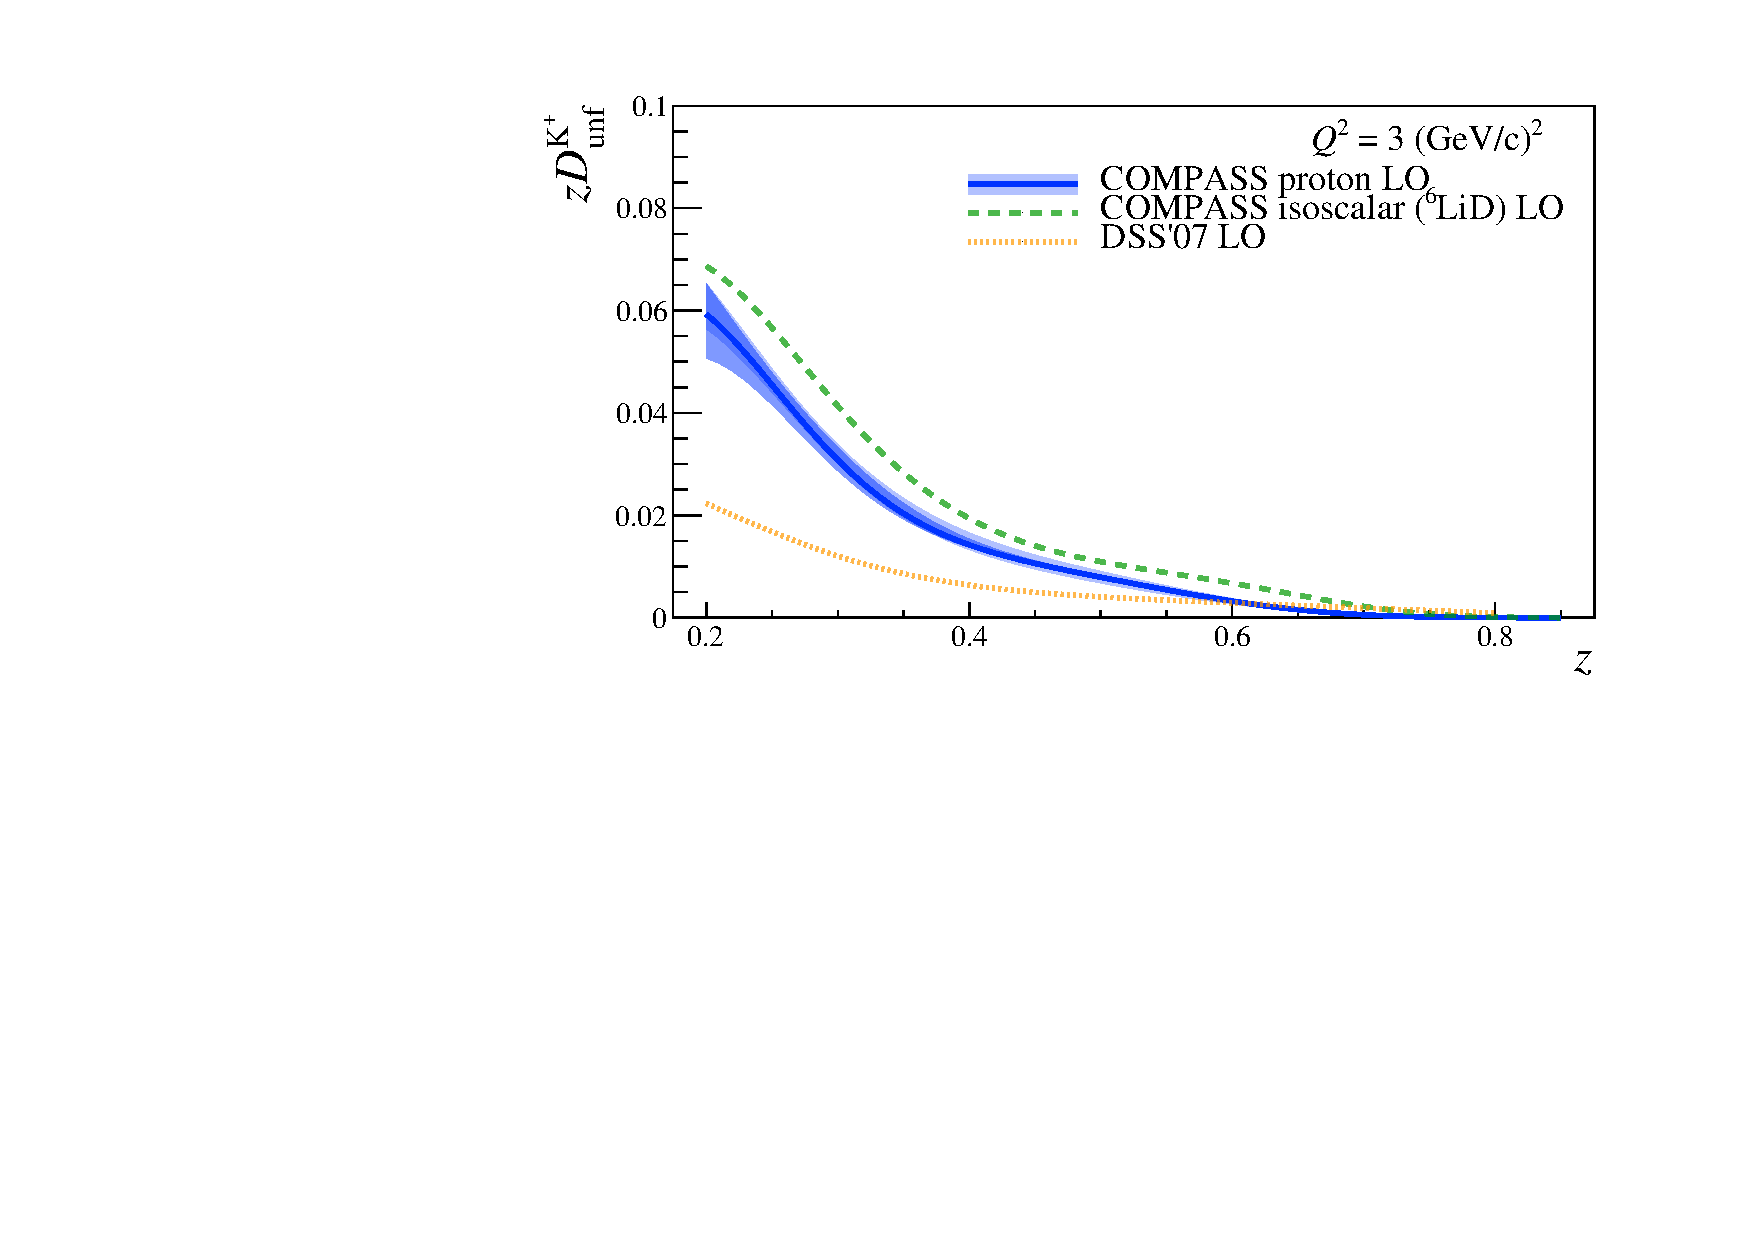
\includegraphics[scale=0.4]{./gfx/unf.pdf}} \\
  \subfloat[$zD^{K}_{s}$]{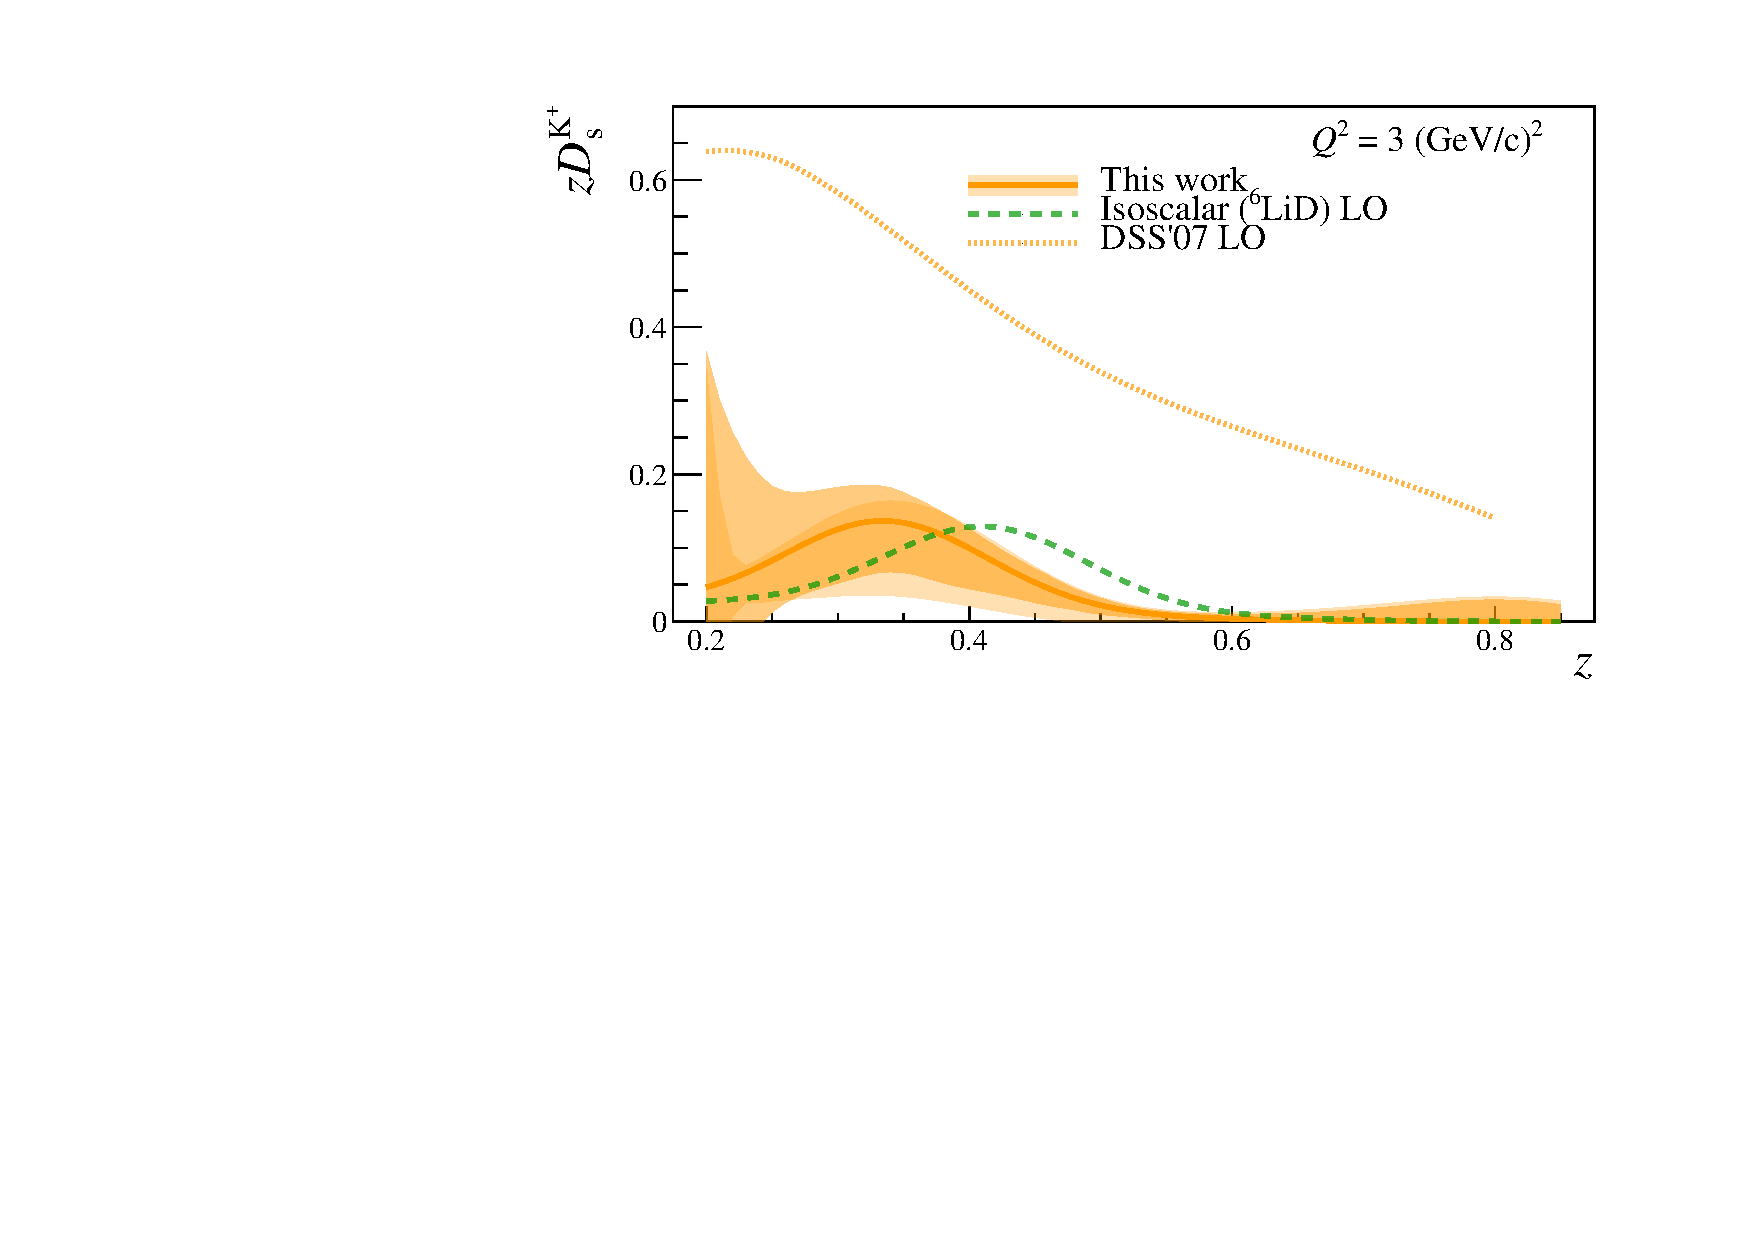
\includegraphics[scale=0.4]{./gfx/sbar.pdf}}
  \subfloat[$zD^{K}_{g}$]{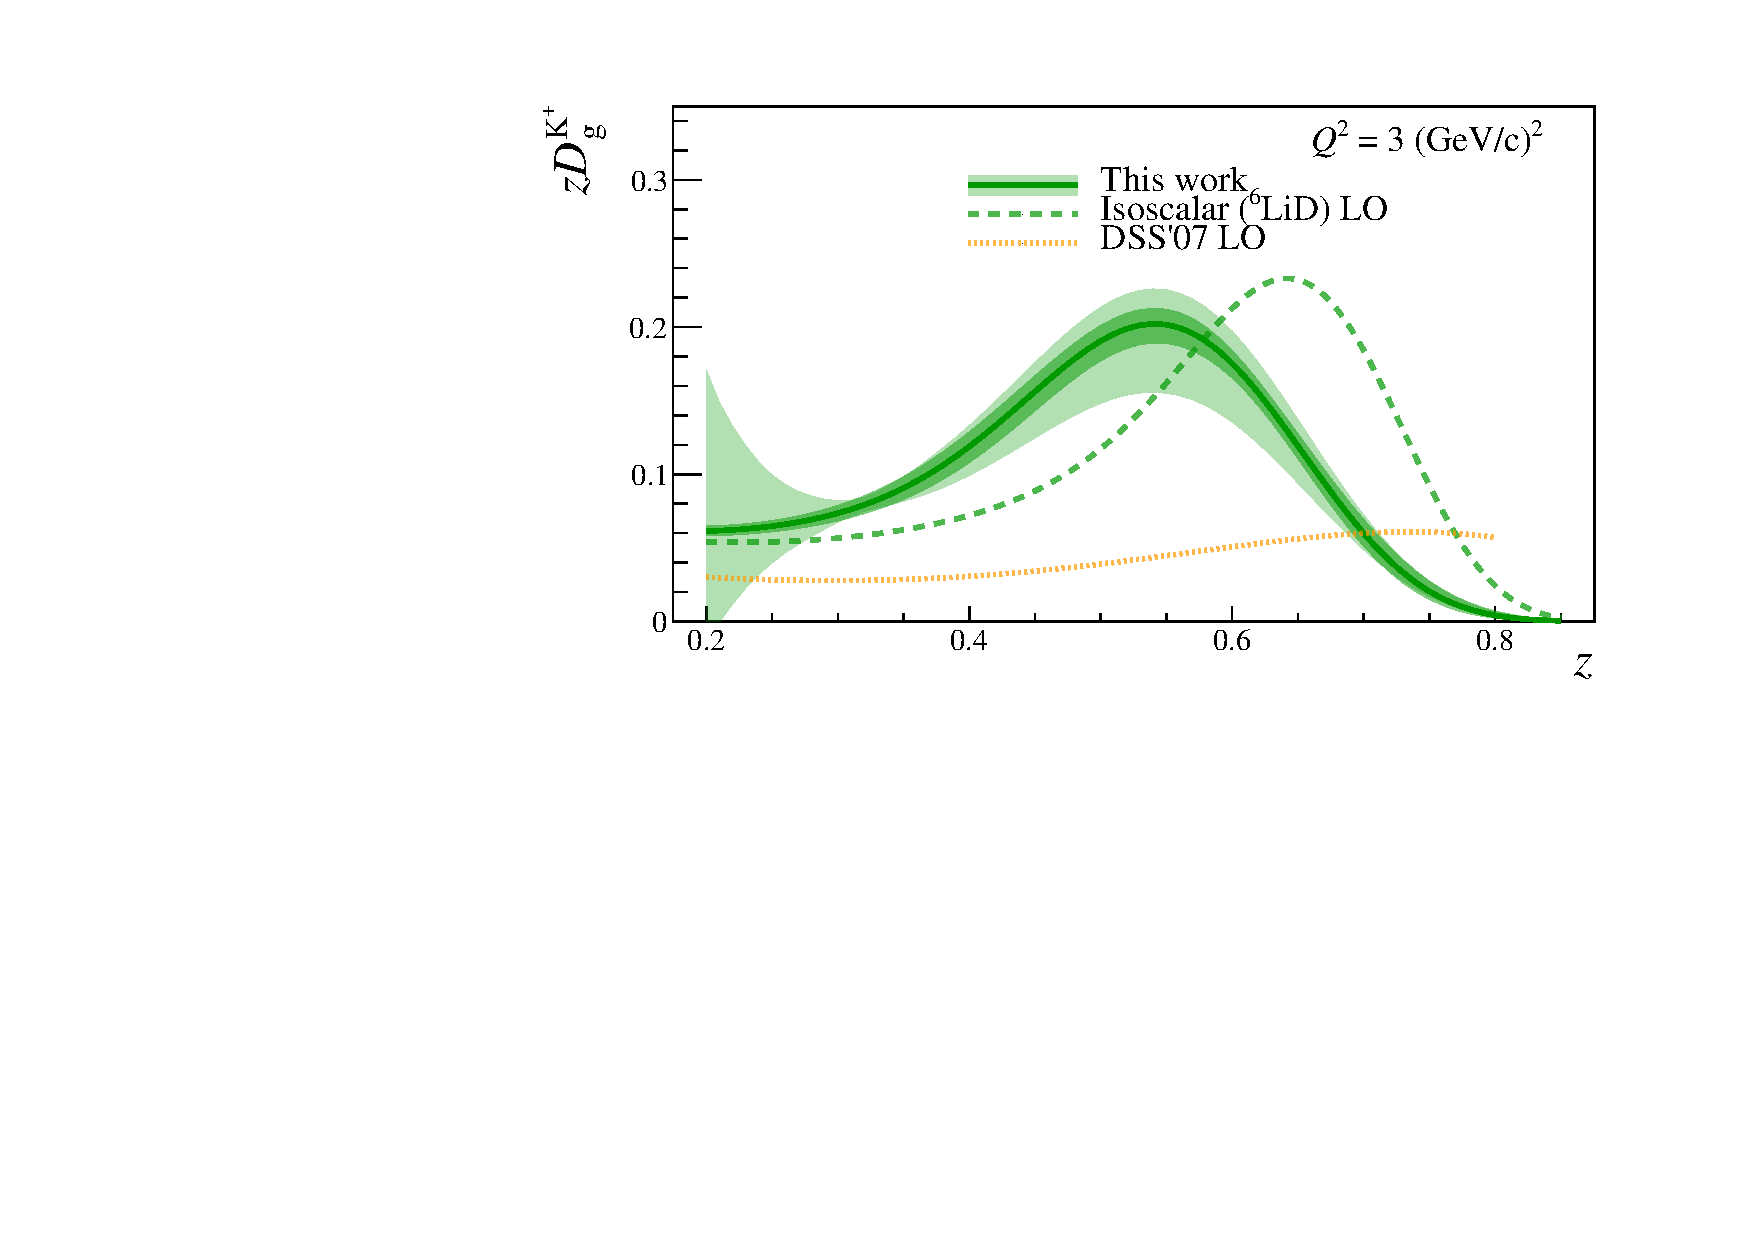
\includegraphics[scale=0.4]{./gfx/gluon.pdf}}
	\caption{The favoured (top left), unfavoured (top right), strange (bottom left) and gluon (bottom right) quark FFs $zD(z)$ into kaons from the COMPASS LO fit. The fit is done based on both the statistical and systematic errors. The green dashed lines are from the same COMPASS LO fit but with COMPASS results for an isoscalar target. The orange dashed line is DSS$07$ LO fit.}
	\label{pic:FFFit}
\end{figure}

%----------------------------------------------------------------------------------------
